\section{Computing a rectification function}

This paper considers single-fix rectification of integer arithmetic circuits. We define single-fix rectification as follows:

\begin{Definition}
Single  fix-rectification  at  target  net $x_i$ means  that  there  exists  a  polynomial  function $U(X_{PI})$ which,  when implemented  at  net $x_i$,  ensures  that circuit $C$ correctly implements the specification $f$.
\end{Definition}

In \cite{utkarsh:fmcad18}, a rectification check theorem (Theorem V.1) was presented to confirm if a net $x_i$ admits single-fix rectification. This rectification check was presented for finite field arithmetic circuits. However, this theorem can be extended to the model used for integer arithmetic circuits. In this paper, we assume that the theorem is applied to a net $x_i$, where single-fix rectification is found to be possible. Given such a net $x_i$, we compute a rectification polynomial which can be implemented at that net to rectify the circuit. 

% \subsection{Problem Statement}

% \begin{itemize}
%     \item Given $R = \Q[x_1,\dots,x_n]$.
%     \item Given a word-level specification polynomial $f$.
%     \item Given a buggy $k$-bit integer multiplier circuit $C$. The bit-level primary inputs are $\{a_0,\dots,a_{k-1}\}$ and $\{b_0,\dots,b_{k-1}\}$. The bit-level primary outputs are $\{z_0,\dots,z_{2k-1}\}$.
%     \item Analyze the topology of the circuit and derive RTTO.
%     \item Given a system of polynomial equations modeling the gates in the circuit $C$, $F=\{f_1,\dots,f_s\}\subset R = \Q[x_1,\dots,x_n]$ and the set $F_0=\{x_1^2-x_1,\dots,x_n^2-x_n\}$.
%     \item Given a net $x_i$ which admits single-fix rectification.
% \end{itemize}

% Our goal is to find a polynomial function $x_i = U(X_{PI})$ that maps $\{0,1\}^{|X_{PI}|} \rightarrow \{0,1\}$, such that $f \in \langle f_1,\dots,f_i:x_i-U(X_{PI}),\dots,f_s,x_1^2-x_1,\dots,x_n^2-x_n \rangle$. This polynomial function rectifies the circuit.

\subsection{Procedure to compute rectification function}

Let $R = \Q[x_1,\dots,x_n]$ and let $F = \{f_1,\dots,f_i:x_i-U(X_{PI}),\dots,f_s\}$ the system of polynomials modeling the correct circuit and $U(X_{PI})$ is the unknown rectification polynomial to be computed. The polynomials are ordered such that according to RTTO, $lt(f_1) > lt(f_2) > \dots > lt(f_i):x_i > lt(f_{i+1}) > \dots > lt(f_s)$. The desired rectification function $U(X_{PI})$ computed must satisfy the condition $f \in \langle f_1,\dots,f_i:x_i-U(X_{PI}),\dots,f_s,x_l^2-x_l \rangle$, where $x_l \in X_{PI}$. This polynomial function $U(X_{PI})$ can be computed using the combination of extended \Grobner Basis and ideal membership testing.

Let the polynomial $f_i = x_i-U$ correct the circuit, where $U$ is a Boolean polynomial. We can write:
\vspace{-1mm}
\begin{equation}
\label{eq:eqn1}
\begin{split}
   f \in \langle & f_1,\dots,f_{i-1},\boldsymbol{f_i: x_i - U},f_{i+1},\dots,f_s, \\
   & x_l^2-x_l \rangle 
\end{split}
\end{equation}

The ideal membership relation of $f$ can be written as:
\vspace{-0.5mm}
\begin{equation}
    \label{eq:eqn2}
\begin{split}
f = & h_1f_1 + h_2f_2 + \dots+\boldsymbol{h_if_i}+\dots+h_sf_s \\
& + \sum_{x_l \in X_{PI}} H_l
\cdot(x_l^2-x_l)    
\end{split}
\end{equation}

where $\{h_1,\dots,h_s,H_l\} \subset R$ are arbitrary polynomials. Substituting $f_i = x_i - U$:
\vspace{-1mm}
\begin{equation}
\begin{split}
    f = & h_1f_1 + h_2f_2 + \dots+\boldsymbol{h_i(x_i-U)}+\dots+h_sf_s \\
    & + \sum_{x_l \in X_{PI}} H_l \cdot(x_l^2-x_l)
\end{split}
\end{equation} 

\begin{equation}
\begin{split}
 f = & h_1f_1 + h_2f_2 + \dots+\boldsymbol{h_ix_i-h_iU}+\dots+h_sf_s \\
 & + \sum_{x_l \in X_{PI}} H_l \cdot(x_l^2-x_l)   
\end{split}
\label{eq:eqn3}
\end{equation}

\begin{equation}
\label{eq:eqn4}
\begin{split}
   & f - h_1f_1 - h_2f_2 - \dots-h_ix_i \\
   & = -h_iU+\dots+h_sf_s + \sum_{x_l \in X_{PI}} H_l \cdot(x_l^2-x_l) 
\end{split}
\end{equation}

Notice that on the L.H.S. of Eqn. (\ref{eq:eqn4}), the polynomials
$f, f_1,\dots,f_{i-1}$ and the monomial $x_i$ are known polynomial expressions. Therefore, $f$ can be divided by $f_1,\dots,f_{i-1}$ and $x_i$ to obtain the respective quotients of the division
$h_1,\dots,h_i$ and remainder $r$. The polynomial $f$ can be written as 
\begin{equation}
f = h_1f_1 + h_2f_2 + \dots + h_ix_i + r
\end{equation}
The remainder $r$ can be computed as:
\begin{equation}
r = f - h_1f_1 - h_2f_2 - \dots - h_ix_i
\label{eq:eqnr}
\end{equation}

After $h_i$ is computed (as quotient of division by $x_i$),
the R.H.S. of Eqn. (\ref{eq:eqn4}) consists of $h_i,f_{i+1},\dots,f_s$ and polynomials $x_l^2-x_l$ as known expressions. This
implies:
\vspace{-1mm}
\begin{equation}
f - h_1f_1 - \dots-h_ix_i \in \langle -h_i,f_{i+1},\dots,f_s,  x_l^2-x_l\rangle
\end{equation}
\vspace{-4mm}
\begin{equation}
r \in \langle -h_i,f_{i+1},\dots,f_s,  x_l^2-x_l\rangle
\label{eq:eqn5}
\end{equation}

Note that RTTO renders the polynomial $f_{i+1},\dots,f_s$ a \Grobner Basis. However, $\{-h_i,f_{i+1},\dots,f_s\}$ is not. We compute its a \Grobner Basis $G = \{g_1,\dots, g_t\}$. We apply the extended \Grobner Basis theory explained in Eqn. (\ref{eqn:imt_orig}) to $G$ to find the ideal membership relation of $r$.

\begin{equation}
    r = -h_i'h_i+h_{i+1}'f_{i+1}+\dots+h_s'f_s+ \sum_{x_l \in X_{PI}} H_l' (x_l^2-x_l)
    \label{eq:eqn6}
\end{equation}

Then $h_i'$ is a polynomial that satisfies the ideal membership relation in Eqn. (\ref{eq:eqn1}). This polynomial rectifies the circuit such that the circuit matches the specification. 

The rectification polynomial $h_i'$ is computed over the field of rational numbers $\Q$. This polynomial may have fractional coefficients. This polynomial may also evaluate to any value in $\Q$ for some primary input vectors. We use the example of a 3-bit multiplier shown in Fig. \ref{fig:3appmult} to explain this in more detail. 

\begin{figure}[H]
    \centering
    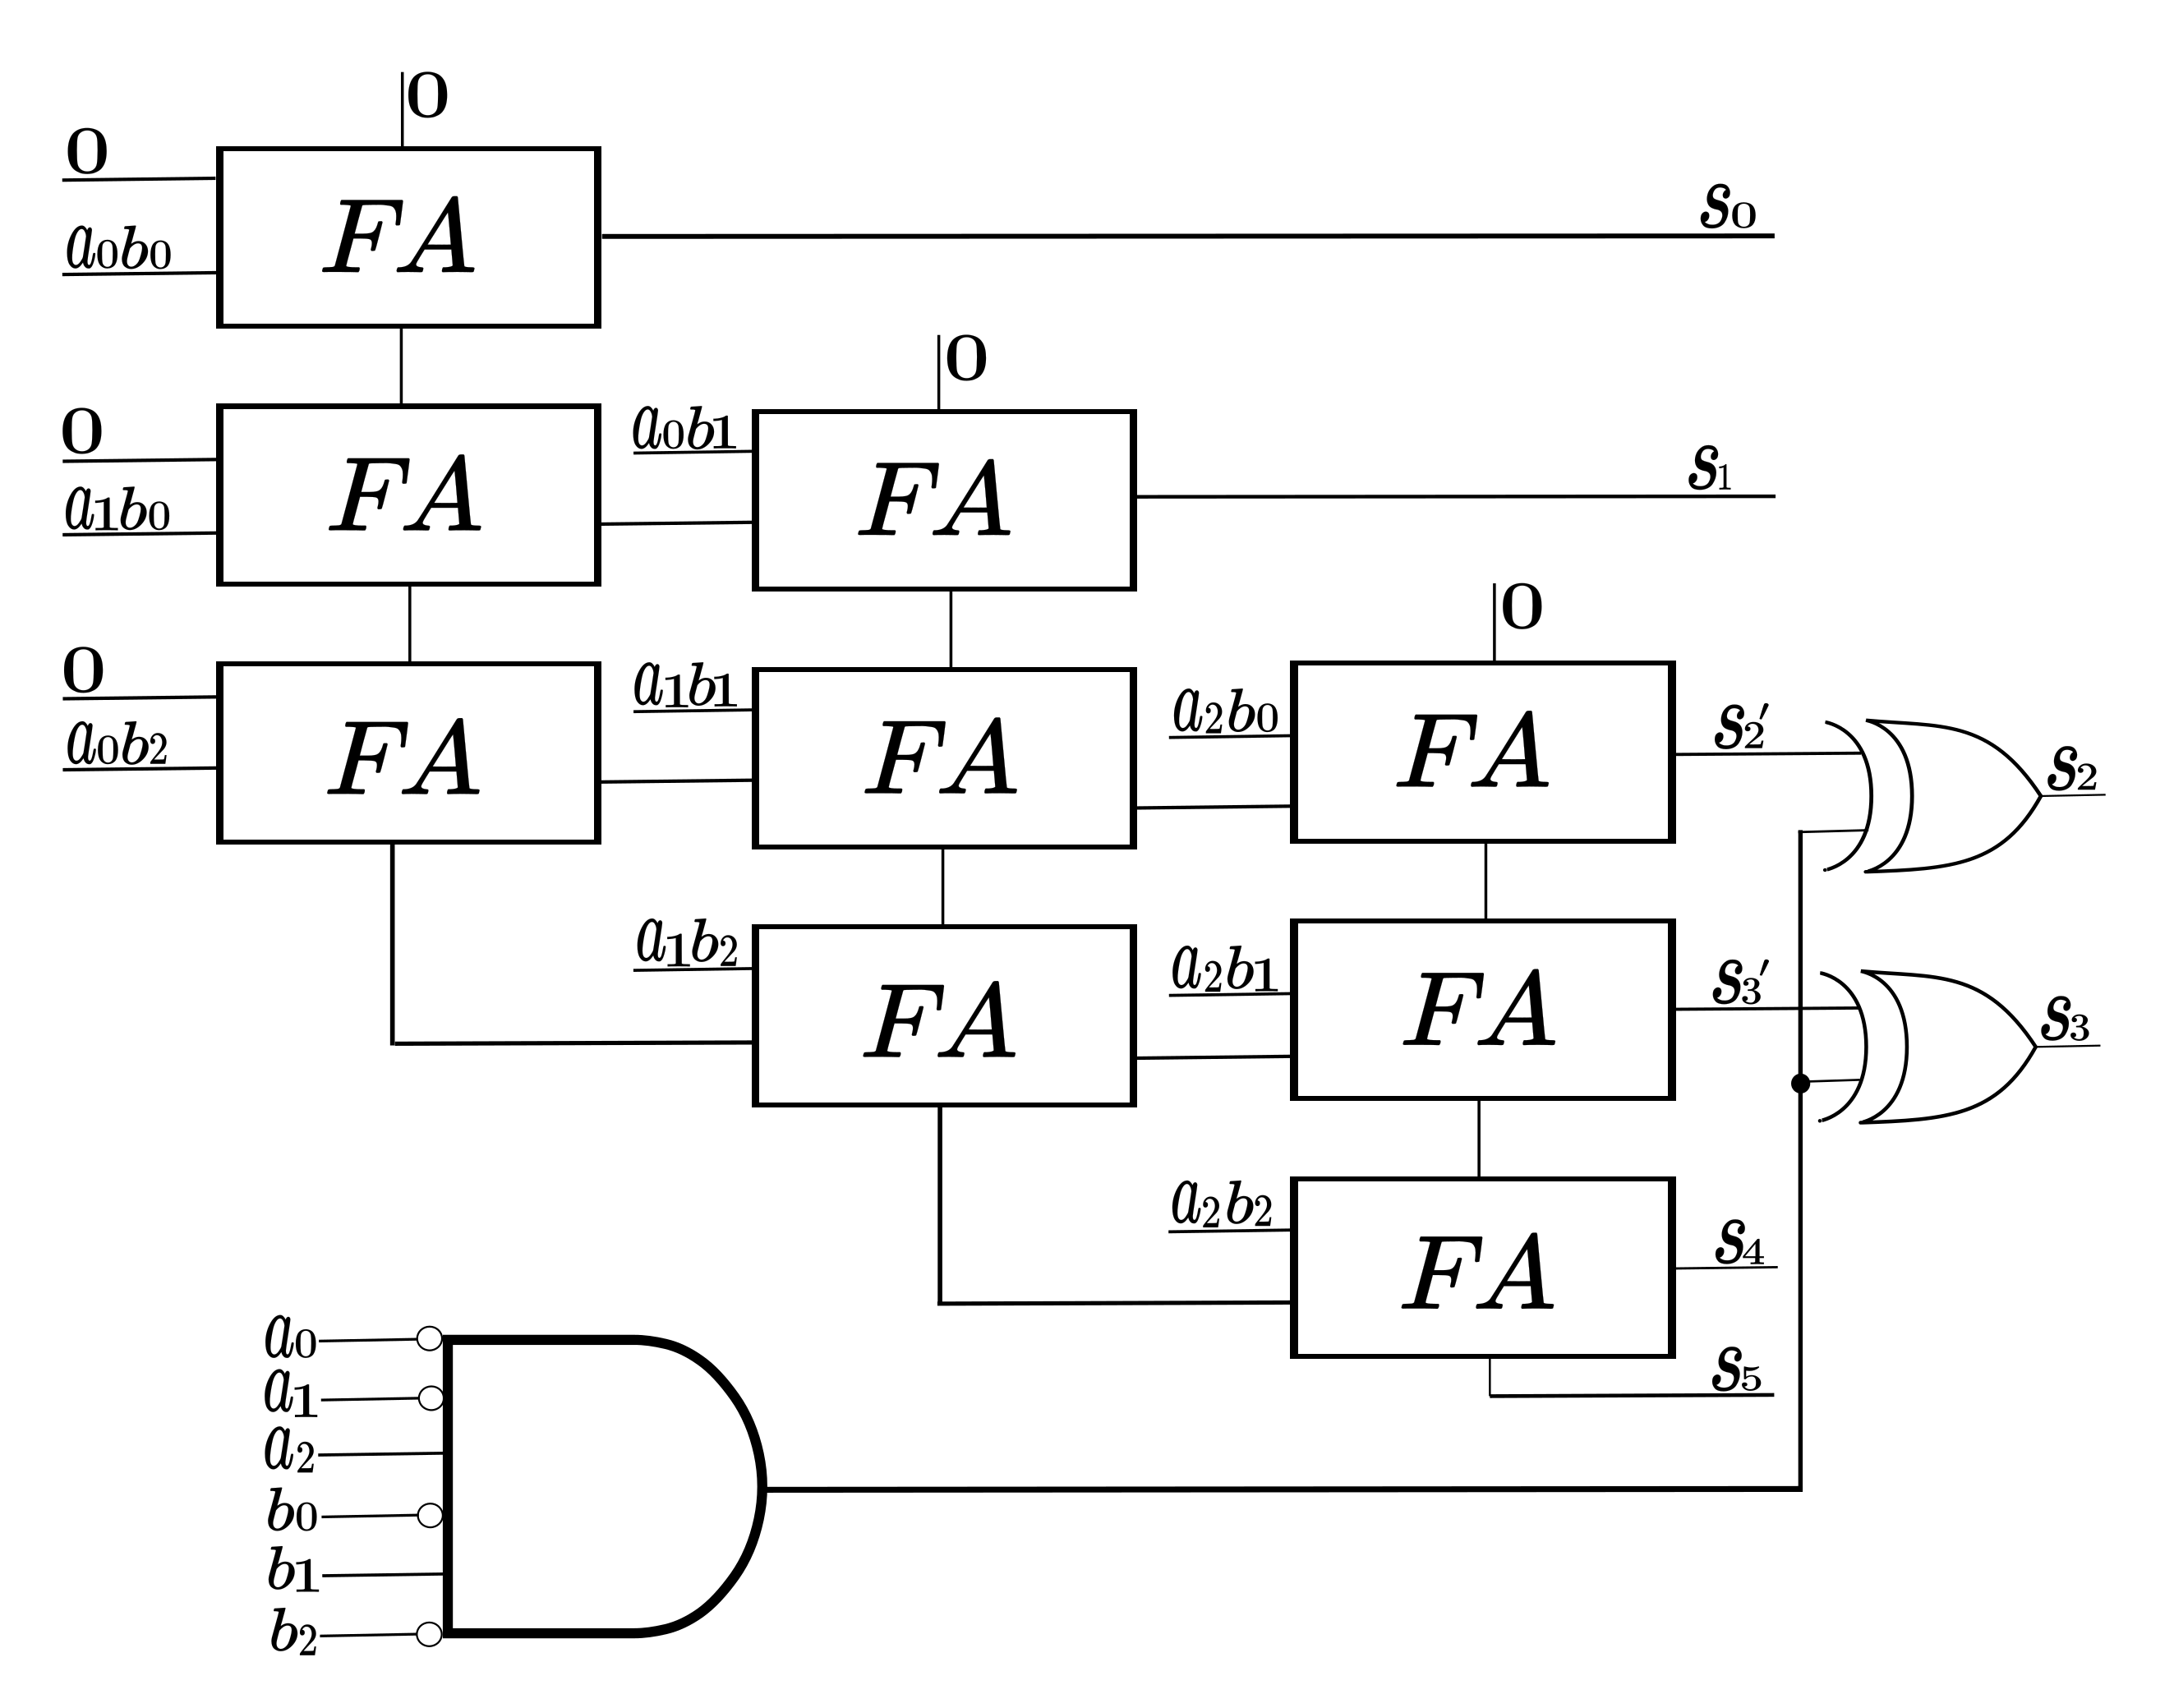
\includegraphics[scale = 0.09]{3appmult.png}
    \caption{3-bit multiplier with additional circuit to introduce a bug}
    \label{fig:3appmult}
\end{figure}

\begin{Example}
The Fig. \ref{fig:3appmult} shows a 3-bit array multiplier circuit. A bug in introduced in the circuit in the form of additional gates as shown. Gates are added to the circuit to modify the function of the circuit at two output bits for one input pattern. We find that single-fix rectification is feasible at a net $n_{22}$ in the circuit. We apply Eqns. (\ref{eq:eqn1}) to (\ref{eq:eqn6}) and compute the rectification function. The following rectification function is computed. We also computed $h_i$ as the quotient of division by $x_i$, as shown in Eqn. (\ref{eq:eqn4}).

\begin{equation}
    \begin{split}
h_i & = 8\cdot a_0\cdot a_1\cdot a_2\cdot b_0
+16\cdot a_0\cdot a_1\cdot a_2\cdot b_1
-12\cdot a_0\cdot a_1 \\
& -8\cdot a_0\cdot a_2\cdot b_0 
 -16\cdot a_0\cdot a_2\cdot b_1 
 +12\cdot a_0-8\cdot a_1\cdot a_2\cdot b_0 \\
& -16\cdot a_1\cdot a_2\cdot b_1 
+12\cdot a_1+8\cdot a_2\cdot b_0
+16\cdot a_2\cdot b_1
-12        
    \end{split}
    \nonumber
\end{equation}

\begin{equation}
    \begin{split}
h_i' = & -\frac{44}{3}\cdot a_0\cdot a_1\cdot a_2\cdot b_0\cdot b_1\cdot b_2+
\frac{4}{3}\cdot a_0\cdot a_1\cdot a_2\cdot b_0\cdot b_1 \\
& +8\cdot a_0\cdot a_1\cdot a_2\cdot b_0\cdot b_2
+\frac{8}{3}\cdot a_0\cdot a_1\cdot a_2\cdot b_1\cdot b_2 \\
& +\frac{4}{3} \cdot a_0\cdot a_1\cdot b_0\cdot b_1\cdot b_2
-\frac{2}{3}\cdot a_0\cdot a_1\cdot b_0\cdot b_1 \\
&+\frac{4}{3}\cdot a_0\cdot a_1\cdot b_1\cdot b_2
+\frac{8}{3}\cdot a_0\cdot a_2\cdot b_0\cdot b_1\cdot b_2 \\
& -4\cdot a_0\cdot a_2\cdot b_0\cdot b_2 
+\frac{28}{3}\cdot a_1\cdot a_2\cdot b_0\cdot b_1\cdot b_2 \\
& -\frac{14}{3}\cdot a_1\cdot a_2\cdot b_0\cdot b_1
-\frac{8}{3}\cdot a_1\cdot a_2\cdot b_0\cdot b_2 \\
&-\frac{20}{3}\cdot a_1\cdot a_2\cdot b_1\cdot b_2
+\frac{8}{3}\cdot a_1\cdot a_2\cdot b_1
-\frac{2}{3}\cdot a_1\cdot b_1 \\
&-\frac{4}{3}\cdot a_1\cdot b_2
+1        
\end{split}
\nonumber
\end{equation}

We evaluate the polynomial $h_i$ and $h_i'$ for all primary input patterns. The observations are recorded in the following table. 
\vspace{2mm}
\begin{table}[ht]
    \centering
    \begin{tabular}{|c|c|c|} \hline
      $a_0,a_1,a_2,b_0,b_1,b_2$ & $h_i$ & $h_i'$ \\ \hline
       0,0,0,0,0,0 & -12 & 1\\ \hline
       0,0,0,0,0,1 & -12 & 1\\ \hline
       0,0,0,0,1,0 & -12 & 1\\ \hline
       0,1,0,0,0,1 & 0 & $-\frac{1}{3}$\\ \hline
       0,1,0,0,1,0 & 0 & $\frac{1}{3}$\\ \hline
       0,1,0,0,1,1 & 0 & -1 \\ \hline
    \end{tabular}
    \caption{Evaluating $h_i$ and $h_i'$}
    \label{tab:quosol}
\end{table}

In order to conserve space, Table \ref{tab:quosol} shows the data for only some input patterns. We make some observations based on the contents of this table. The rectification polynomial $h_i'$ has fractional coefficients. At points where $h_i = 0$, we see that $h_i'$ evaluates to any value in $\Q$. We found 48 such points where $h_i$ evaluates to 0. At points where $h_i \neq 0$, we observe that $h_i'$ evaluates to a value in $\{0,1\}$.
\end{Example}

Consider the polynomial $h_i$ which is computed as a quotient of division by $x_i$ in Eqn. (\ref{eq:eqn4}). We can see that the rectification polynomial $h_i'$ depends on the polynomial $h_i$. This is also confirmed by the data shown in Table \ref{tab:quosol}. In order to understand the conditions under which the rectification polynomial $h_i'$ we compute is a Boolean polynomial, we look at the variety of $h_i$.

Let us assume there exists a polynomial $U$, which can be implemented at net $x_i$ to rectify the circuit. This polynomial is a Boolean polynomial, which performs the mapping $\{0,1\}^{|X_j|} \rightarrow \{0,1\}$, where $X_j$ is the set of variable that are less than $x_i$ in RTTO. This polynomial can be reduced to the primary input variables, $U(X_{PI})$. The existence of such a polynomial can be confirmed by performing the rectification check at $x_i$, shown in \cite{utkarsh:fmcad18}. 
% \vspace{2mm}

Based on these assumptions, we state the following facts. 

\begin{Fact}
The polynomial $h_i$ is computed in terms of variables in the set $X_j$, where $X_j < x_i$ in RTTO. 
\end{Fact}

We use \Grobner basis division to compute $h_i$. This division is shown in Eqn. (\ref{eq:eqn4}). The order of division ensures that $h_i$ is a polynomial in those variables which are less than $x_i$ in the term order.

\begin{Fact}
The polynomial $h_i'$ is computed in terms of variables in the set $X_j$, where $X_j < x_i$ in RTTO. 
\end{Fact}

The application of extended \Grobner basis algorithm, being used to compute $h_i'$ in Eqn. (\ref{eq:eqn6}), ensures that $h_i'$ is a polynomial in those variables which are less than $x_i$ in the term order.

\begin{Fact}
\begin{equation}
    h_i(U-h_i') = \sum_{j = i+1}^{s} (h_j-h_j')f_j+\sum_{x_l\in X_{PI}}(H_l-H_l')(x_l^2-x_l)
    \label{eq:eqn7}
\end{equation}
\end{Fact}

We get Eqn. (\ref{eq:eqn7}) by combining Eqns. (\ref{eq:eqn4}), (\ref{eq:eqnr}) and (\ref{eq:eqn6}).

\begin{Fact}
$\forall p \in \{0,1\}^{|X_{PI}|},\ \exists p'$, such that $p'|_{X_{PI}} = p$ and $f_{i+1}(p') = \dots = f_s(p') = 0$.
\end{Fact}

For all primary input assignments, there exists an assignment that satisfies all the gates in the circuit. 

By using the four facts stated above, we propose the following theorem. 

% \begin{Theorem}
% Let point $p \in \{0,1\}^{|X_{PI}|}$ be a point.\\
% (i) If $h_i(p) = 0$, i.e., $p \in V(\langle h_i \rangle + J_0)$, then $h_i'(p)$ evaluates to a value in $\Q$.\\
% (ii) If $h_i(p) \neq 0$, i.e., $p \notin V(\langle h_i \rangle + J_0)$, then $h_i'(p) \in \{0,1\}$.
% \label{thm:quo2}
% \end{Theorem}

\begin{Theorem}
Let there exist a polynomial $U$ that maps from $\{0,1\}^{|X_j|} \rightarrow \{0,1\}$. Let $p'$ be a point such that $p'|_{X_{PI}} = p$ and $f_{i+1}(p') = \dots = f_s(p') = 0$. If $h_i(p') = 0$, then $h_i'(p) = U(p')$.
\label{thm:quo}
\end{Theorem}

\textbf{Proof:}
Consider Eqn. (\ref{eq:eqn7}). Consider a point $p'$ such that $p'|_{X_{PI}}$ and $f_{i+1}(p') = \dots = f_s(p') = 0$. We know that $x_l^2 = x_l$ at any point $p \in \{0,1\}^{|X_{PI}|}$. Therefore, R.H.S. of Eqn. (\ref{eq:eqn7}) is 0.

\begin{equation}
    h_i(U - h_i') = 0. 
    \label{eq:hi0}
\end{equation}
In L.H.S. of Eqn. (\ref{eq:hi0}), since $h_i(p') \neq 0$, $U(p') = h_i'(p')$. 

Since we know that $U$ is a Boolean polynomial, we know that $U(p')$ is a value in $\{0,1\}$. Therefore, according to Theorem \ref{thm:quo}, $h_i'$ evaluates to a Boolean value at those points where $h_i \neq 0$. 

\begin{Corollary}
Let point $p$ be such that $p \in \{0,1\}^{|X_{PI}|}$. Let $p'$ be a point such that $p'|_{X_{PI}} = p$. If $h_i(p') = 0$, the polynomial $h_i'$ can be modified such that $h_i'(p')$ evaluates to a value in $\{0,1\}$.
\end{Corollary}

\textbf{Proof:} Consider Eqn. (\ref{eq:eqn7}). Consider a point $p'$ such that $p'|_{X_{PI}}$ and $f_{i+1}(p') = \dots = f_s(p') = 0$. We know that $x_l^2 = x_l$ at any point $p \in \{0,1\}^|X_{PI}|$. Therefore, R.H.S. of Eqn. (\ref{eq:eqn7}) is 0.
\begin{equation}
    h_i(U - h_i') = 0. 
    \label{eq:hinot0}
\end{equation}
In L.H.S. of Eqn. (\ref{eq:hinot0}), since $h_i(p') = 0$. Therefore, it does not depend on $h_i'(p')$. 

The corollary for Theorem \ref{thm:quo} implies that we can modify
the polynomial function $h_i'$ at those points $p$, where $h_i(p) = 0$, to evaluate to any
value in $\{0,1\}$, without affecting the ideal membership relation in Eqn (\ref{eq:eqn5}). These points are the local don't cares of the rectification function.

Due to the compact structure of arithmetic circuits, we usually compute polynomial $h_i$ such that $V(\langle h_i \rangle + J_0) = \emptyset$. This implies that the polynomial does not evaluate to 0 at any point in $\{0,1\}^{|X_{PI}|}$. 

\begin{Corollary}
\label{thm:quo2}
If $\forall p \in \{0,1\}^{|X_{PI}|}$ and $h_i(p') \neq 0\ \forall p'$ such that $p'|_{X_{PI}} = p$, then polynomial $U$ is unique and can be computed as polynomial $h_i'$ by application of Eqns. (\ref{eq:eqn1}) to (\ref{eq:eqn6}). 
\end{Corollary}

\textbf{Proof:} By extension of proof for Theorem \ref{thm:quo}, $U(p') = h_i'(p'),\ \forall p'$.

Corollary \ref{thm:quo2} can be explained using the following example of a 2-bit integer multiplier shown in Fig. \ref{fig:2mult}.

\begin{figure}[H]
    \centering
    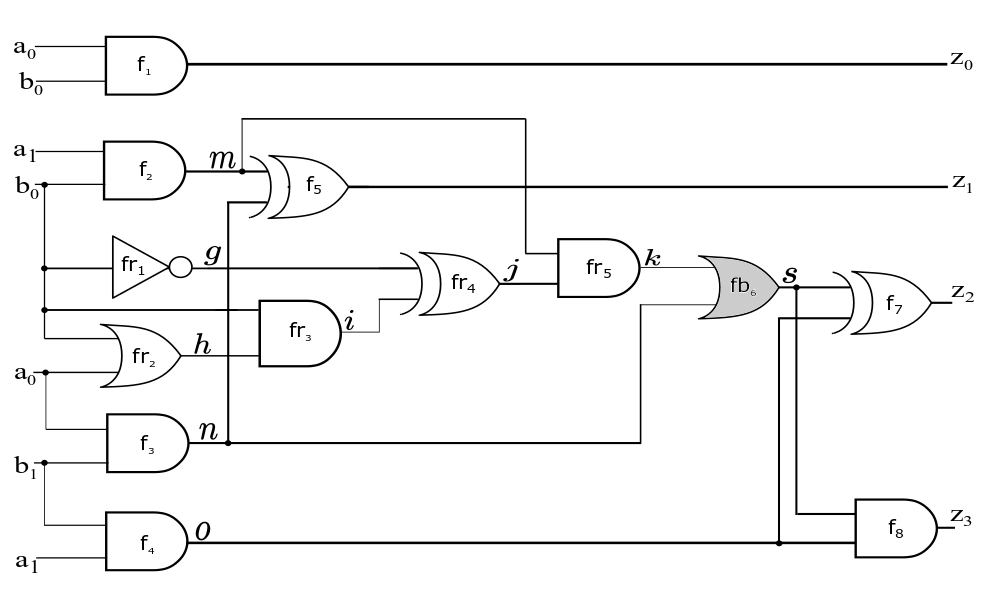
\includegraphics[scale = 0.25]{int_mul_red_b.png}
    \caption{2-bit integer multiplier with redundancy}
    \label{fig:2mult}
\end{figure}
\begin{Example}
A bug is introduced in the circuit shown in Fig. \ref{fig:2mult}. The bug is introduced at net $s$ by replacing the AND gate by an OR gate. Rectification was attempted at net $s$ itself. 
The polynomials for the circuit, with the bug at $s$, are:

\begin{align*}
& f_1 = -z_0+a_0\cdot b_0 && f_2 = -m+a_1\cdot b_0 \\
& f_{r1} = -g+1-b_0 && f_{r2} = -h+a_0+b_0 - a_0\cdot b_0 \\
& f_3 = -n+a_0\cdot b_1 && f_4 = -o+a_1\cdot b_1 \\
& f_5 = -z_1+m+n-2\cdot m \cdot n && f_{r3} = -i+h \cdot b_0 \\
& f_{r4} = -j+i+g-2 \cdot i \cdot g && f_{r5} = -k+j \cdot m \\
& \mathbf{f_{b6} = -s+k+ n-k\cdot n} && f_7 = -z_2+s+o-2\cdot s \cdot o \\
& f_8 = -z_3+s\cdot o \\
\end{align*}

The procedure to compute a rectification polynomial was applied. 

Consider the two polynomials computed.
\vspace{-2mm}
$$h_i =  -8\cdot g\cdot h\cdot n\cdot b_0
+4\cdot g\cdot n
+4\cdot h\cdot n\cdot b_0
-4\cdot n
+2$$ and 
$$h_i' = -n-2\cdot o+a_0\cdot b_1+a_1\cdot b_0+2\cdot a_1\cdot b_1$$

The polynomial $h_i'$ is the rectification polynomial we computed.

Let us reduce the polynomial $h_i$ to primary input variables. Compute $h_i \pmod{J+J_0} = 2$. This clearly indicates that $h_i$ never evaluates to $0$ for any value in $\{0,1\}^{|X_{PI}|}$. 

Consider the polynomial $h_i' = -n-2\cdot o+a_0\cdot b_1+a_1\cdot b_0+2\cdot a_1\cdot b_1$. Let us reduce the polynomial to primary inputs variables. Compute $h_i' \pmod{J+J_0} = a_1 \cdot b_0$. For all values in $\{0,1\}^{|X_{PI}|}$, this polynomial only evaluates to a value in $\{0,1\}$. This indicates that it is a Boolean polynomial. 
\end{Example}







